\documentclass[11pt,a4paper,titlepage]{article}

\usepackage{pdflscape}
\usepackage[margin=1in]{geometry}
\usepackage{titling}
\usepackage{graphicx}
\usepackage{titlesec}
\usepackage[hidelinks]{hyperref}

\graphicspath{ {./Images/} }

\setcounter{secnumdepth}{4}

\titleformat{\paragraph}
{\normalfont\normalsize\bfseries}{\theparagraph}{1em}{}
\titlespacing*{\paragraph}
{0pt}{3.25ex plus 1ex minus .2ex}{1.5ex plus .2ex}

\begin{document}
%\title{ \huge Functional Requirements for the SAMBUG}

\begin{titlepage}
    \centering
    \vfill
    {\bfseries\Huge
        SAMBUG\\
        Master Specification\\
      \hfill\\
         \Large COS 301
        \vskip2cm
        
\includegraphics[width=6cm]{sambug}
        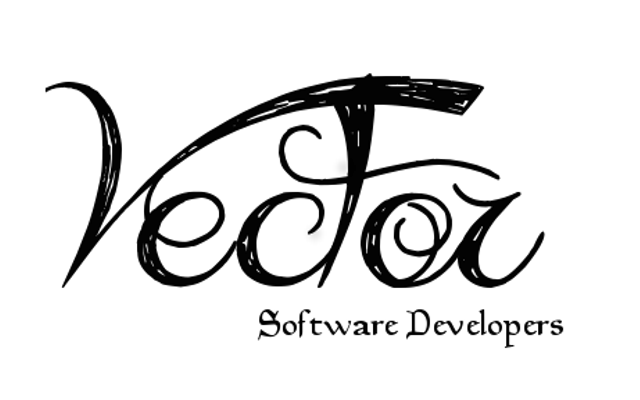
\includegraphics[width=8cm]{logo} \\

    }    
    \vfill
    \begin{tabular}{lr}
        	Abrie van Aardt&13178840\\
		Werner Mostert&13019695\\
		Kale-ab Tessera&13048423\\
		Keagan Thompson&13023782\\
		Michelle Swanepoel&13066294\\
	\end{tabular}
    
    
    \vfill
    \textbf{October 2015}
    \vfill
\end{titlepage}
	
%\author
%{     
%	Abrie van Aardt 13178840\\
%	Werner Mostert 13019695\\
%	Kele-ab Tessera 13048423\\
%	Keagan Thompson 13023782\\
%	Michelle Swanepoel 13066294\\
%}
    
%\date{\textbf{May 2015}}

%\maketitle

\tableofcontents

\pagebreak


% Put all images in images folder - Please use PNG's not Jpegs
% Preferably create separate file for your domain - just like with the use cases
\pagebreak


\section{Background}
South Africa is currently the largest producer of macadamia nuts in the world. One of the main production and quality limiting factors is the incidence of stink bug damage. 
\\Accurate timing of chemical sprays rely on accurate scout data and economic threshold levels of the insect pests in an orchard. However, scouting for these pests has
a major shortfall, namely the accurate identification of pests, despite efforts to train growers and scouts by various means.\\
Area wide control of pests and diseases is a concept that has been considered, but with the lack of scout data from across and within growing regions it is impossible to make such recommendations. \\

\section{Vision}
An innovative approach to handling the management and acquisition of scout data is to develop a smartphone application that is able to identify specific hemipteran species by making use of the built-in camera of the smartphone. This application makes use of the smartphone’s built-in GPS to perform geotagging and uploading information to a central database. In addition to the data management, one of the primary goals is to supply data mining methods on historical data as obtained via the smartphone application. A visual representation of said data is therefore made available in a dynamic and easy way for the every day farmer and researcher.

\section{Scope}
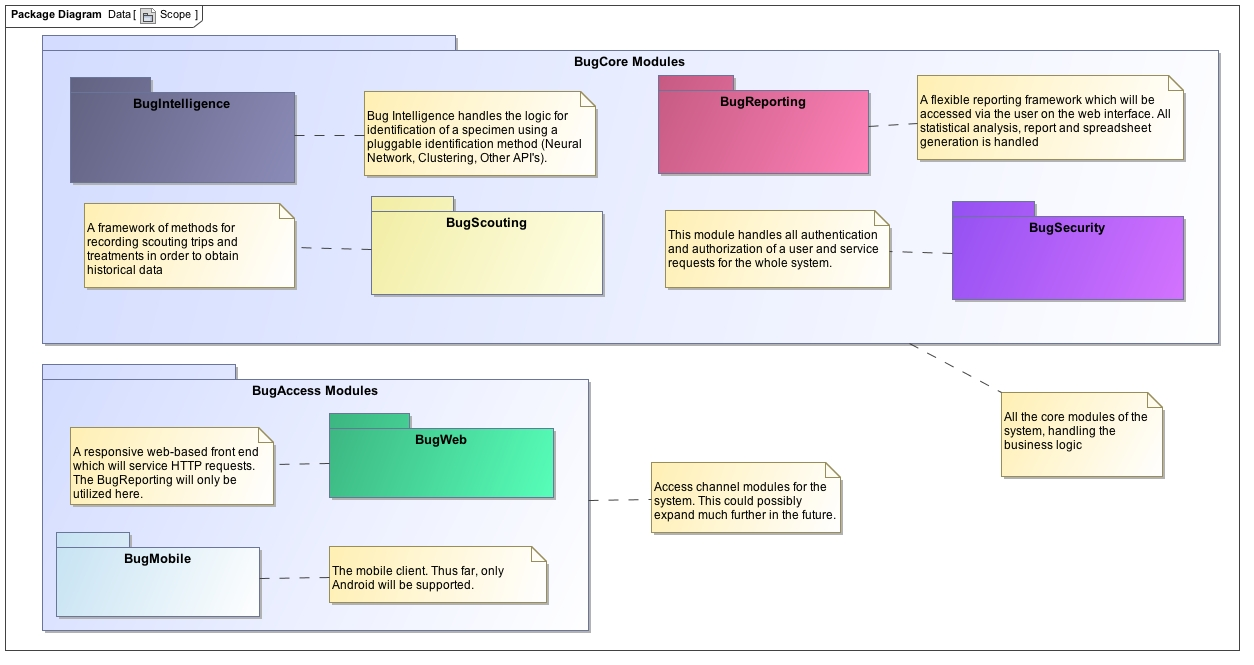
\includegraphics[width=\linewidth]{scope}

%\section{Architecture requirements}
%	\subsection{Access channel requirements}
%	\subsection{Quality requirements}
%	\subsection{Integration requirements}
%	\subsection{Architecture constraints}
\section{Functional Requirements and Application Design}
	\subsection{Domain Model}
		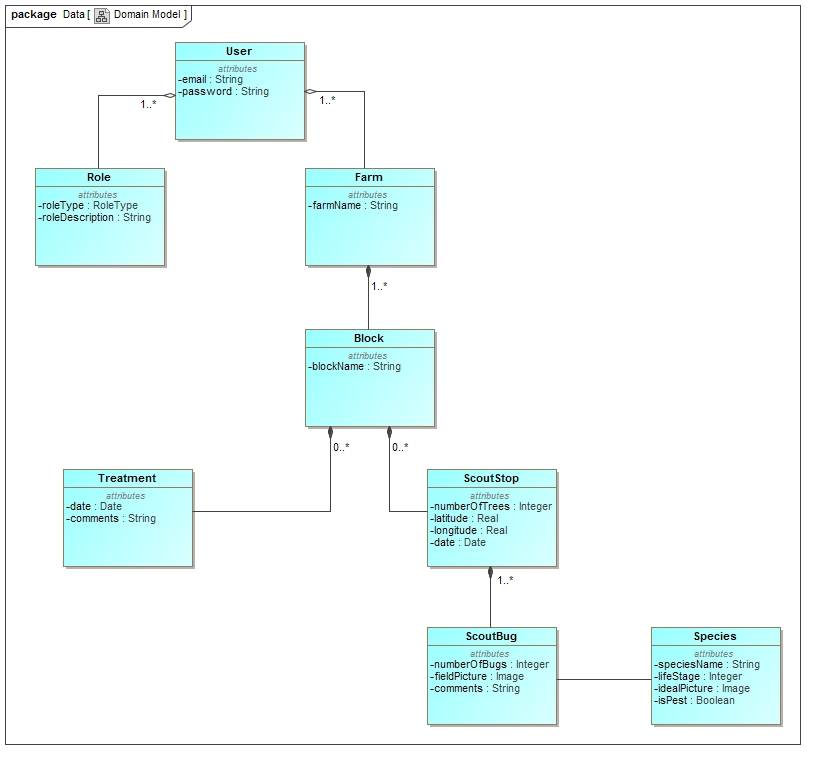
\includegraphics[width=\linewidth]{DomainModel}
%------------------------------------------------------------------------------------------%

	\subsection{BugScouting}
		The BugScouting module has the following functionality:
		\begin{enumerate}
			\item It provides the functionality for a user to be able to enter data related to a scouting trip - entering data such as the number of trees scouted, the number of bugs per tree and the different kind of bugs specified. After this data has been entered, a summary should be displayed for the user.
			\item It provides the ability for a user to record the details related to spraying, such as the date of spraying and the specific block that was sprayed.
		\end{enumerate}

		In many ways this module may be regarded as the "core" functionality of the system. This encompasses the main purpose of the system.
		\subsubsection{Module Scope}
		The scope of the \textit{BugScouting} module is shown below:\\
		\hfill\\
		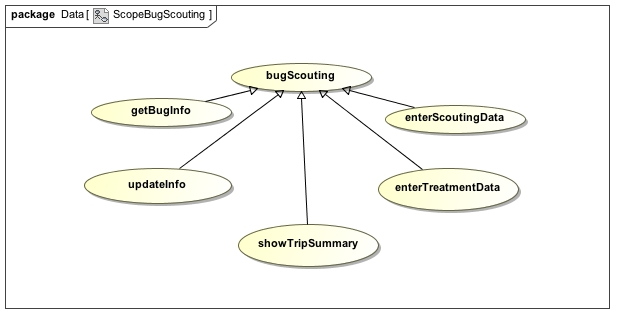
\includegraphics[width=\linewidth]{ScopeBugScouting}
		
		\subsubsection{Use Cases}
		The concrete use cases for the \textit{BugScouting} module follow:
		\paragraph{getBugInfo \dotfill [Priority - Medium]}
		This use case uses the BugIntelligence module to retrieve information on a specific specimen which will be used to display to the user a "wiki" like piece which has the purpose of informing the user.\\\hfill\\
		The Service Contract for the \textit{getBugInfo} use case is shown below:\\\hfill\\
		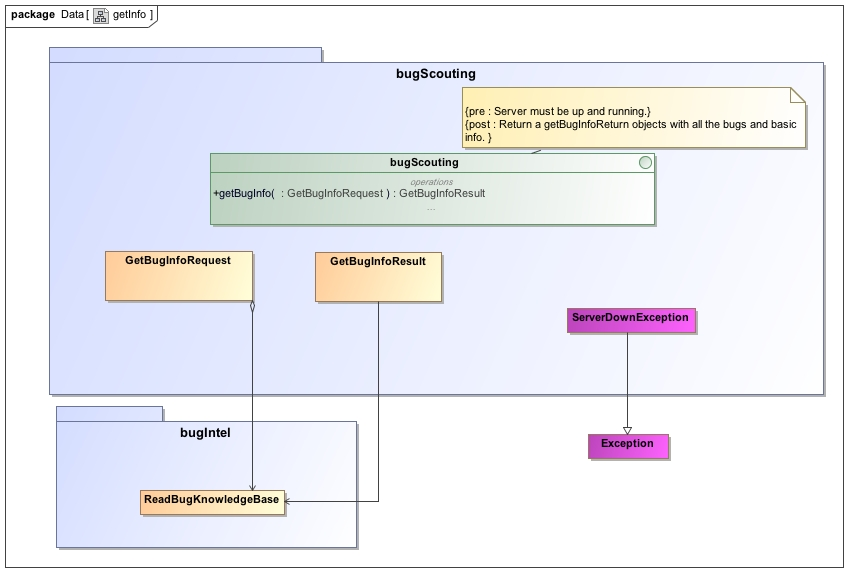
\includegraphics[width=\linewidth]{getInfo}
		
		\paragraph{updateInfo \dotfill [Priority - Medium]}
		The objective of this use case is to provide functionality to retrieve updated bug information and identification method updates.\\\hfill\\
		The Service Contract for the \textit{getBugInfo} use case is shown below:\\\hfill\\
		\includegraphics[width=\linewidth]{updateInfo}
		
		\paragraph{showTripSummary \dotfill [Priority - High]}
		After completing a full scouting trip, this use case should provide a summary of the entire scouting trip. One scouting trip may consist of many scouting stops and each scout stop may include the finding of various bugs. The averages for the scouting trip data is used in the summary.\\\hfill\\
		The Service Contract for the \textit{showTripSummary} use case is shown below:\\\hfill\\
		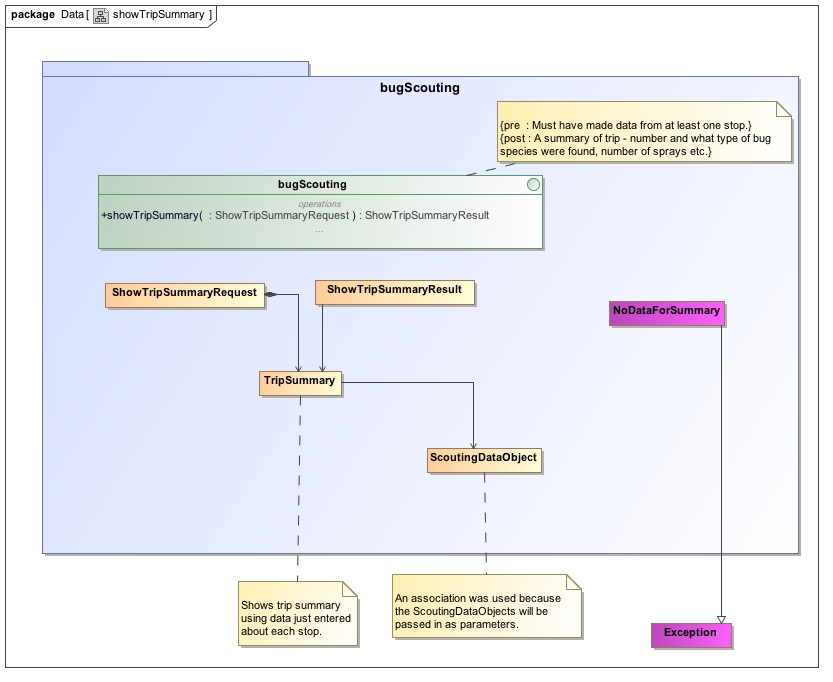
\includegraphics[width=\linewidth]{showTripSummary}
		
		\paragraph{enterTreatmentData \dotfill [Priority - Critical]}
		This use case is for entering data related to spraying chemicals (pesticide). This allows for the type of chemical, the date and the block or orchard number to be recorded.\\\hfill\\
		
		The Service Contract for the \textit{enterTreatmentData} use case is shown below:\\\hfill\\
		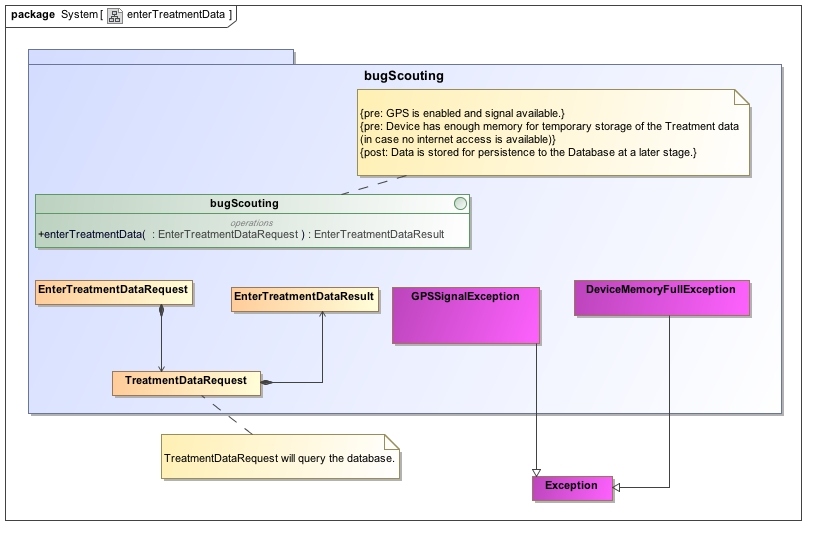
\includegraphics[width=\linewidth]{EnterTreatmentData}
		
		\paragraph{enterScoutingData \dotfill [Priority - Critical]}
		This is the core use case of this module. This use case allows entering data related to a scouting stop. Data captured should include the number of trees observed, the number of bugs encountered and the block number where the scouting took place. After entering the data, the specimen should be identified (classified), either manually or automatically, before successfully submitting it for persistence.\\\hfill\\
		The Service Contract for the \textit{enterScoutingData} use case is shown below:\\\hfill\\
		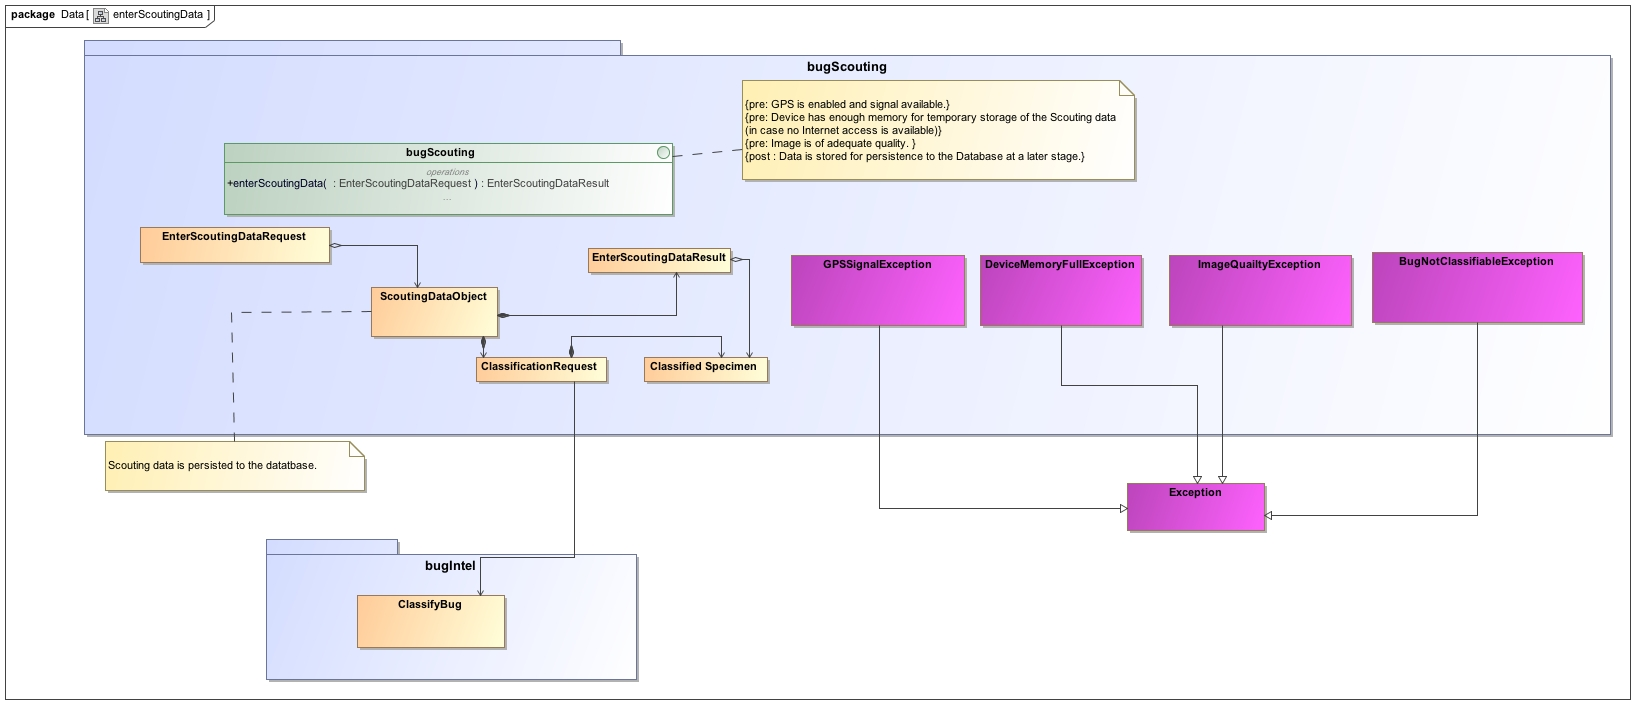
\includegraphics[width=\linewidth]{enterScoutingData}
		The Process Specification for the \textit{enterScoutingData} use case is shown below:\\\hfill\\
		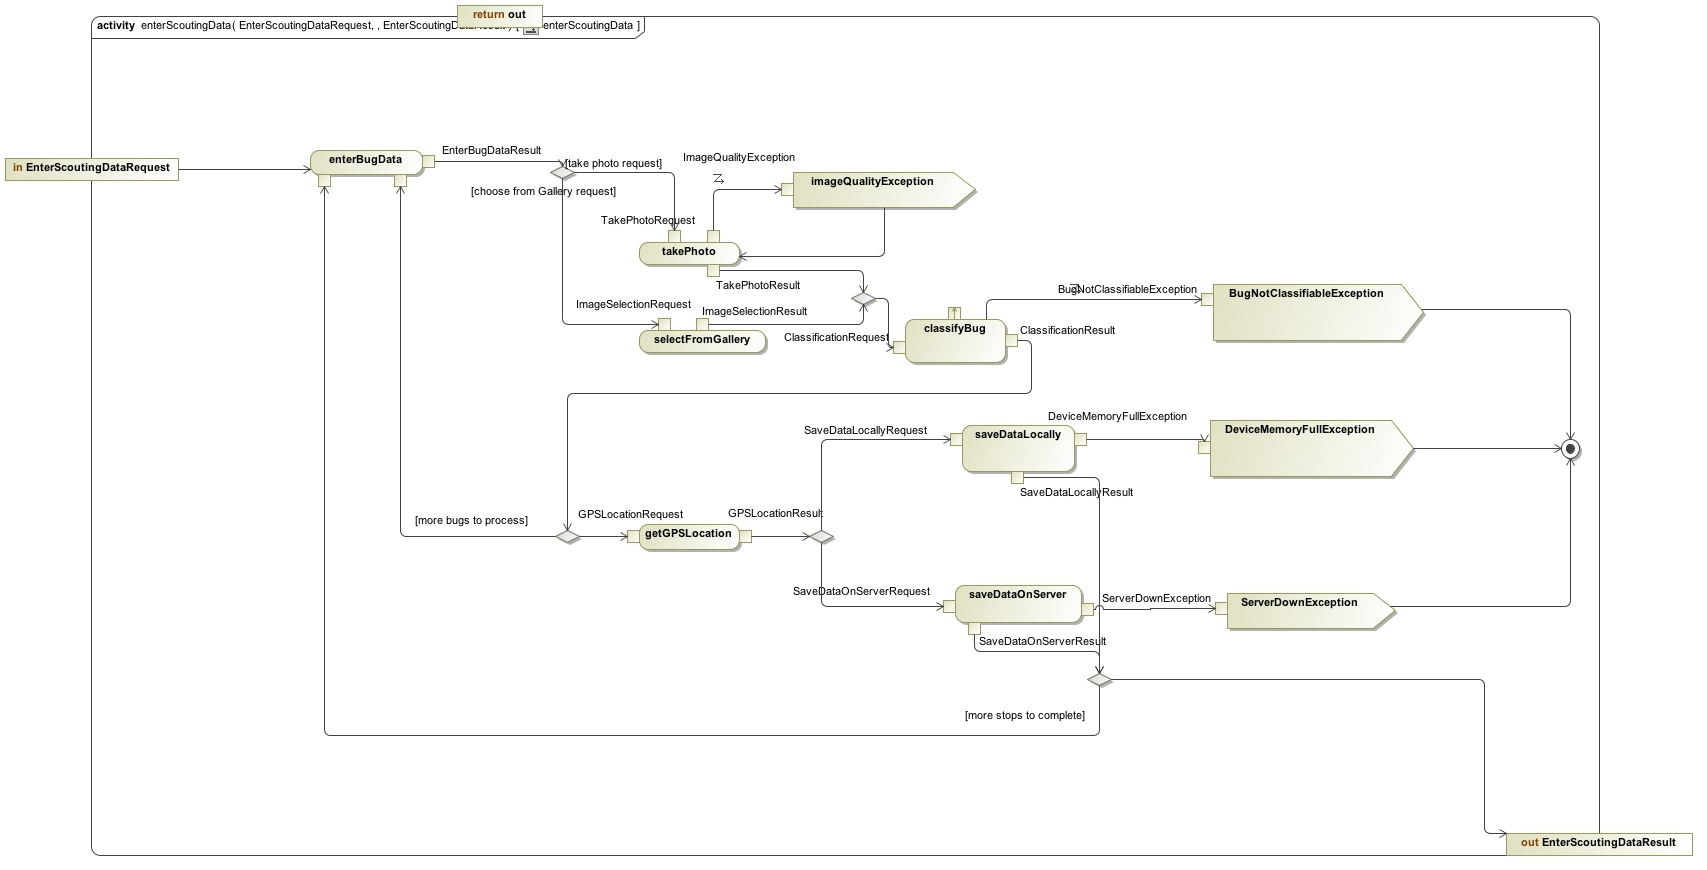
\includegraphics[width=\linewidth]{enterScoutingDataPS}
		
		
		
		
%------------------------------------------------------------------------------------------%	
	
	\subsection{BugIntelligence}
		The BugIntelligence module has the following functionality:
		\begin{enumerate}		
			\item It provides a pluggable method to classify a specimen according to species and life stage.
			\item It provides an interface which can be used to obtain information related to any specific specimen which is identifiable by the system
			\item It provides CRUD(Create Read Update Delete) functionality for bug information for specimens identifiable by the identification method
		\end{enumerate}
		\subsubsection{Module Scope}
		The scope of the \textit{BugIntelligence} module is shown below:\\
		\hfill\\
		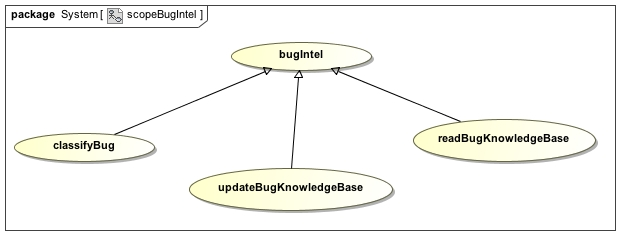
\includegraphics[width=\linewidth]{scopeBugIntel}
		\subsubsection{Use Cases}
		The concrete use cases for the \textit{BugIntelligence} module follow:
		
		\paragraph{classifyBug \dotfill [Priority - Critical]}
		This use case supplies a method to classify the bug according to life stage and species. The classification method used is pluggable.\\\hfill\\
		The Service Contract for the \textit{classifyBug} use case is shown below:\\\hfill\\
		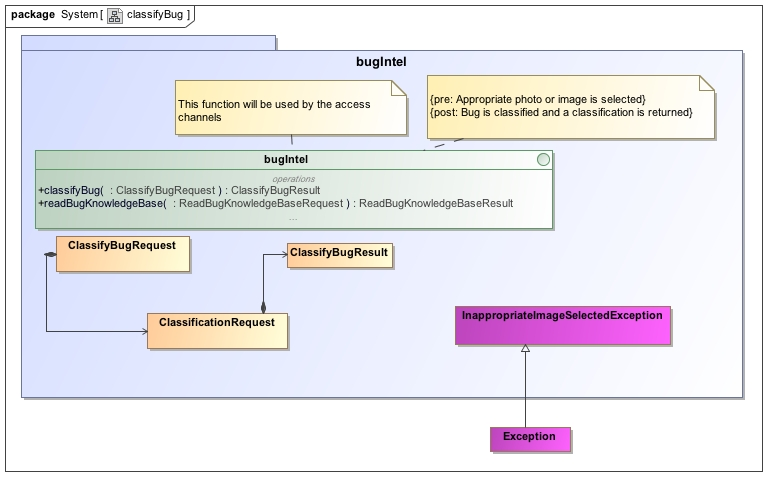
\includegraphics[width=\linewidth]{classifyBug}
		
		The Process Specification for the \textit{classifyBug} use case is shown below:\\\hfill\\
		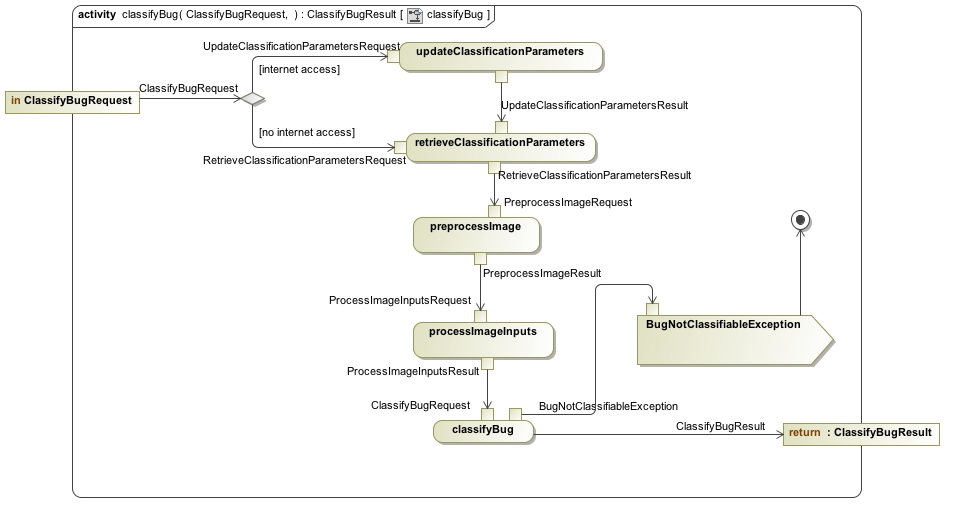
\includegraphics[width=\linewidth]{classfyBugPS}
		
		\paragraph{updateBugKnowledgeBase \dotfill [Priority - Low]}		
		This use case provides the functionality to edit the information used for classification. As in the example of a neural network being used as a classification method, the training examples may be edited.		
		The Service Contract for the \textit{updateBugKnowledgeBase} use case is shown below:\\\hfill\\
		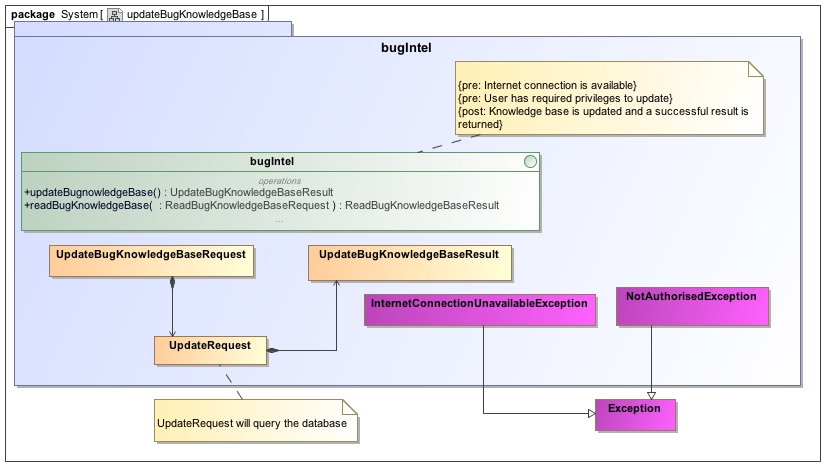
\includegraphics[width=\linewidth]{updateBugKnowledgeBase}
		
		\paragraph{readBugKnowledgeBase \dotfill [Priority - Critical]}
				This use case provides the functionality to get the information used for classification. As in the example of a neural network being used as a classification method, the training examples may be retrieved.	
		The Service Contract for the \textit{readBugKnowledgeBase} use case is shown below:\\\hfill\\
		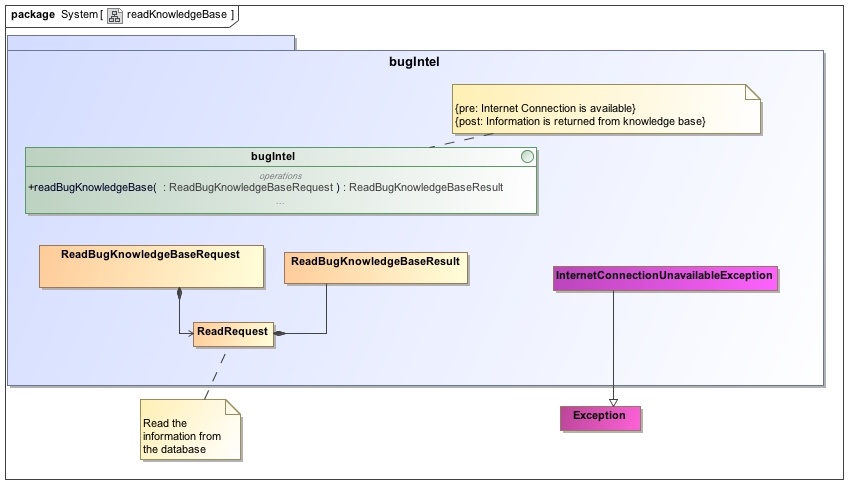
\includegraphics[width=\linewidth]{readKnowledgeBase}
		
		
%------------------------------------------------------------------------------------------%		
	\subsection{BugSecurity}
	The BugSecurity module allows the following functionality:
	\begin{enumerate}
		\item It provides functionality related to user accounts and user roles in order to login, register and recover your account within the capacity of a user role.
		\item It provides functionality to determine whether a specific service request should be allowed.
	\end{enumerate}
		\subsubsection{Module Scope}
		The scope of the \textit{BugSecurity} module is shown below:\\
		\hfill\\
		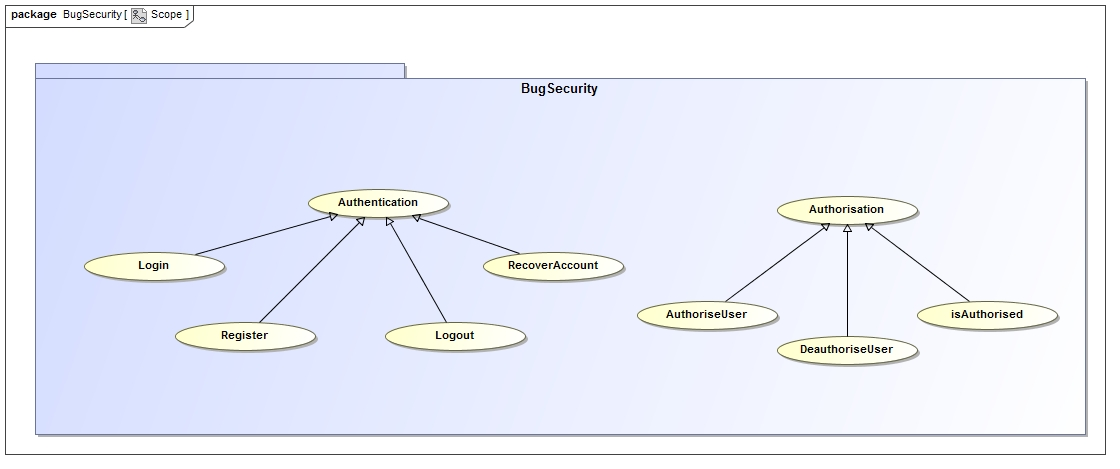
\includegraphics[width=\linewidth]{SecurityScope}
		\subsubsection{Use Cases}
		The concrete use cases for the \textit{BugSecurity} module follow:
		
		\paragraph{login \dotfill [Priority - Critical]}
		This use cases allows one to login with username and password credentials which will be validated and thus allowing the user to be authenticated.\\\hfill\\
		The Service Contract for the \textit{login} use case is shown below:\\\hfill\\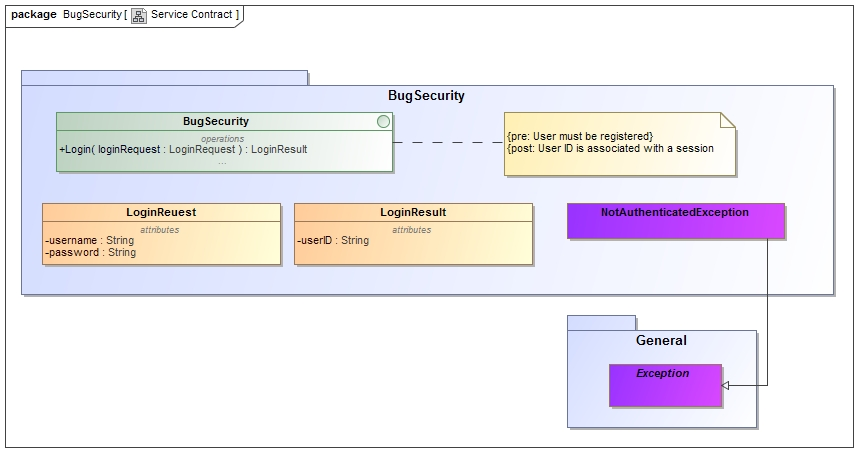
\includegraphics[width=\linewidth]{LoginSC}
		
		\paragraph{register \dotfill [Priority - Critical]}
		This use case caters for registration as a new user. A user account is created which is associated with a unique user name. Currently, there are no password format requirements.\\\hfill\\
		The Service Contract for the \textit{register} use case is shown below:\\\hfill\\
		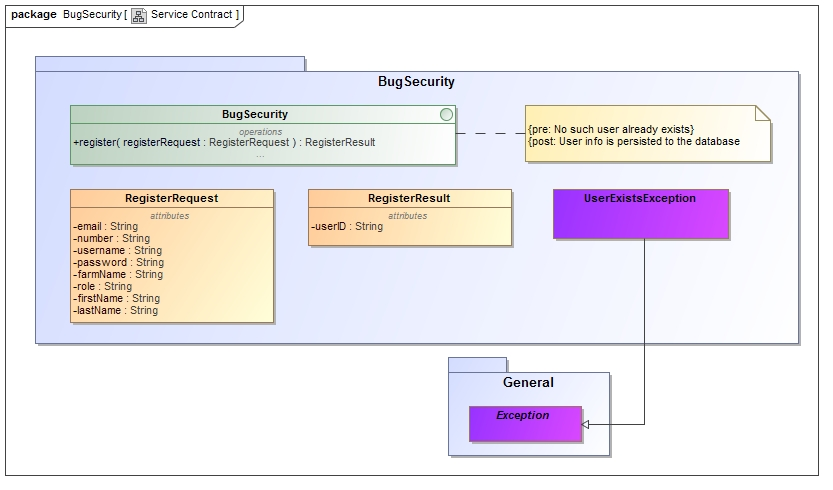
\includegraphics[width=\linewidth]{RegisterSC}		
		
		\paragraph{logout \dotfill [Priority - Medium]}
		This use case provides functionality to log out of the system.\\\hfill\\
		The Service Contract for the \textit{logout} use case is shown below:\\\hfill\\
		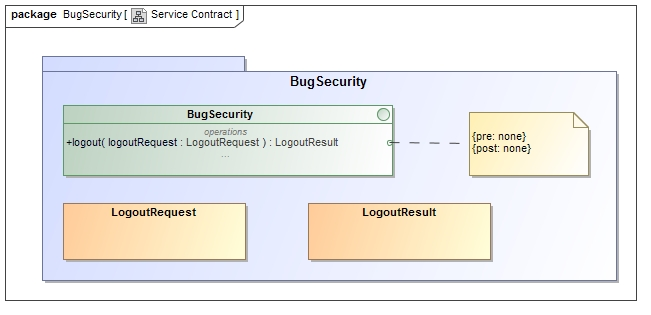
\includegraphics[width=\linewidth]{LogoutSC}
		
		\paragraph{recoverAccount \dotfill [Priority - Low]}
		In the case where a user forgets or has lost his/her credentials to access the system, this use case provides functionality to recover or to generate a new password. User verification is done via the email address associated with the account.\\\hfill\\ 
		The Service Contract for the \textit{recoverAccount} use case is shown below:\\\hfill\\
		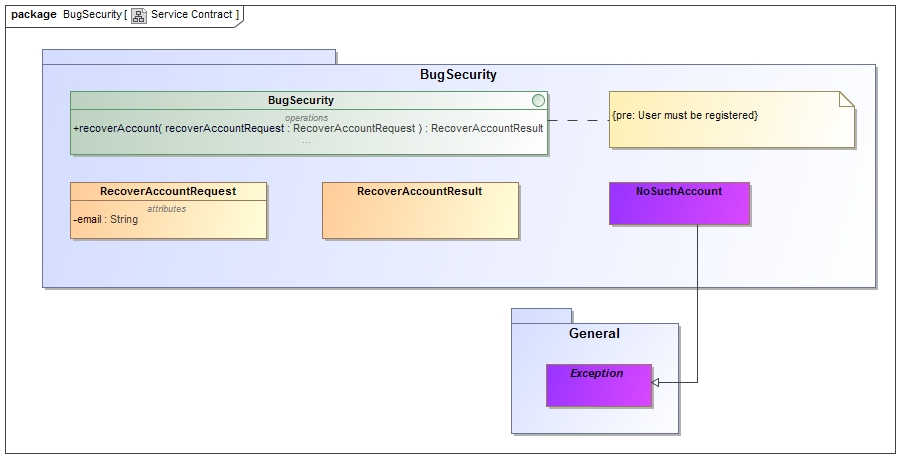
\includegraphics[width=\linewidth]{RecoverAccountSC}
		
		\paragraph{isAuthorised \dotfill [Priority - High]}
		Whenever a service which should not be accessibility to entire plethora of users is requested, authorization is required. This use case makes provision for this.\\\hfill\\
		The Service Contract for the \textit{isAuthorised} use case is shown below:\\\hfill\\
		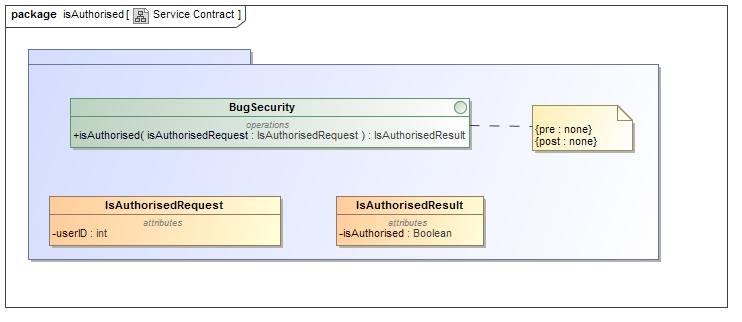
\includegraphics[width=\linewidth]{isAuthorised}
		\paragraph{authoriseUser \dotfill [Priority - Medium]}
		This use case allows for an authorization restriction for a service to be added/\\\hfill\\
		The Service Contract for the \textit{authoriseUser} use case is shown below:\\\hfill\\
		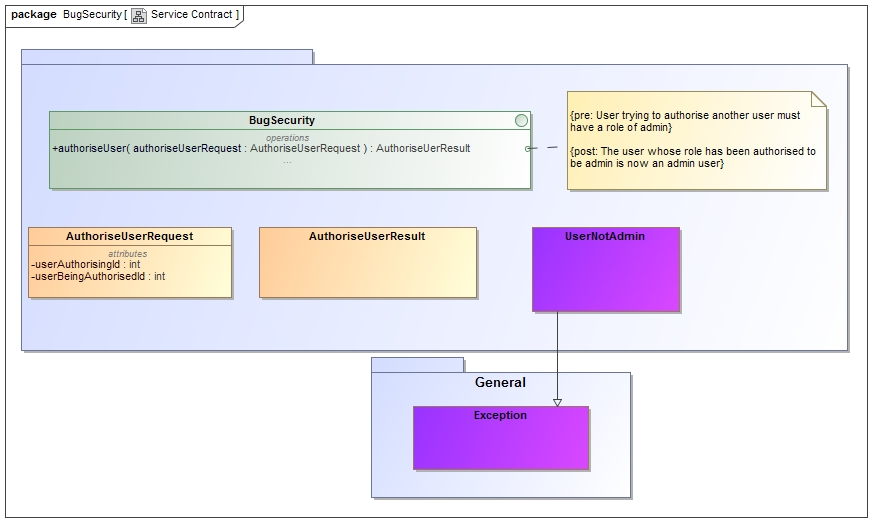
\includegraphics[width=\linewidth]{authorise}
		\paragraph{deauthoriseUser \dotfill [Priority - Medium]}
				This use case allows for an authorization restriction for a service to be removed/\\\hfill\\
		The Service Contract for the \textit{deauthoriseUser} use case is shown below:\\\hfill\\
		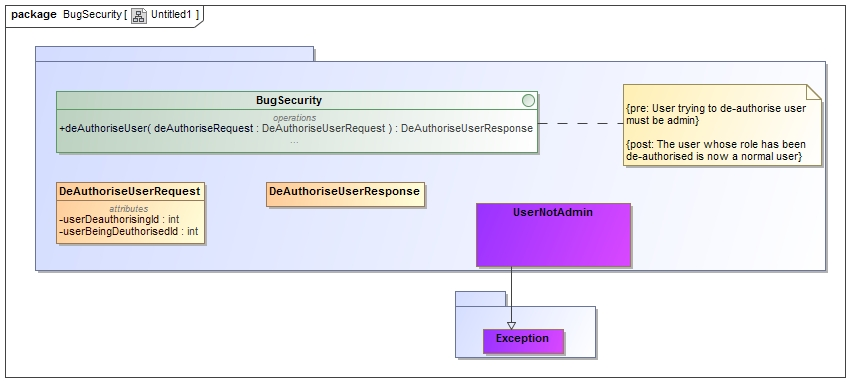
\includegraphics[width=\linewidth]{deauthor}
		
		
		
%------------------------------------------------------------------------------------------%		
	\subsection{BugReporting}
	The BugReporting module allows the following functionality:
	\begin{enumerate}
		\item It provides functionality to generate historical data in a usable, tabular - as used by Microsoft Excel and similar software, format.
		\item It provides functionality to generate a visual representation of historical data in the form of a dynamically chosen set of graphs.
		\item It provides functionality to generate a heat map of the farm with regards to the population of stink bugs identified.
	\end{enumerate}
		\subsubsection{Module Scope}
		The scope of the \textit{BugReporting} module is shown below:\\
		\hfill\\
			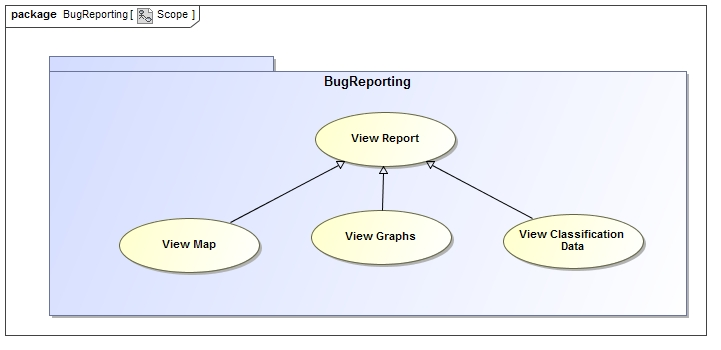
\includegraphics[width=\linewidth]{ReportingScope}
		\subsubsection{Use Cases}
		The concrete use cases for the \textit{BugReporting} module follow:
		\paragraph{viewMap \dotfill [Priority - Medium]}
		This use case provides the functionality to view a heat map, where the total number of pests found will be shown. Areas with more pests will show a darker area on the map. One will this be able to conclude which areas are experiencing a problem with pests. Multiple constraints and filters can be applied to show only a subset of the data available.\\\hfill\\
		The Service Contract for the \textit{viewMap} use case is shown below:\\\hfill\\		
		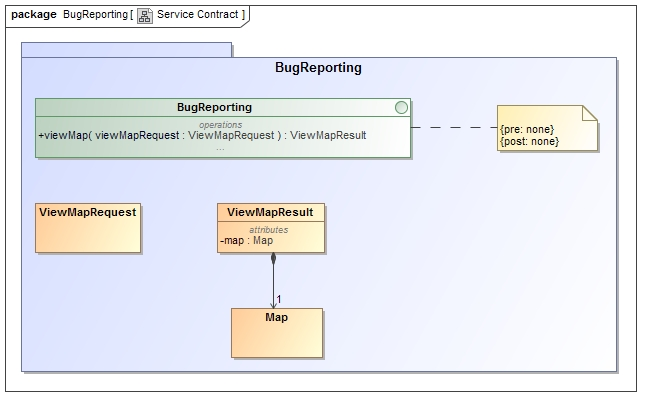
\includegraphics[width=\linewidth]{viewMapSC}
		
		\paragraph{viewCharts \dotfill [Priority - Medium]}
		This use case provides the functionality to view data that was collected through the mobile application, specifically sccouting data. The data will be displayed in the form of dynamic charts, where one can choose multiple filters and constraints to apply to the data. One will be able to see how spraying affects the pest count.\\\hfill\\
		The Service Contract for the \textit{viewCharts} use case is shown below:\\\hfill\\	
		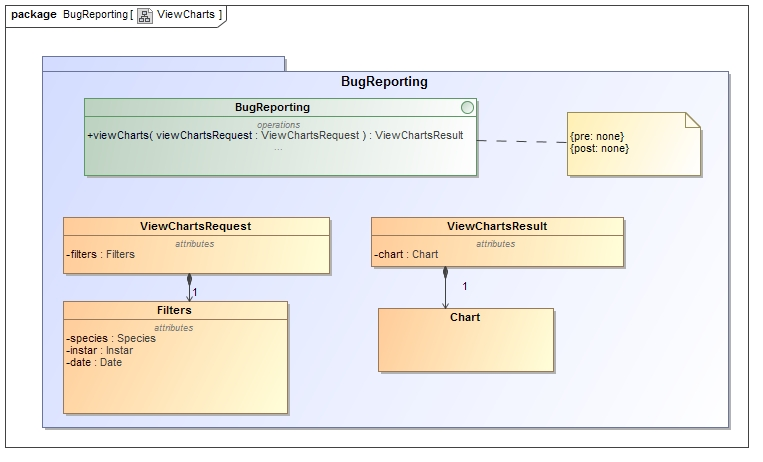
\includegraphics[width=\linewidth]{viewCharts}	
		
		\paragraph{viewTables \dotfill [Priority - Medium]}
		This use case allows the user to see data that has been collected through the mobile application, specifically scouting data. The data will be displayed in the form of a table and will have the functionlity to download this as an Excel spreadsheet, PDF document or to print the table. One will be able to also view spraying data. Multiple filters and constraints can be applied to the data to only view a subset of the data available.\\\hfill\\
		The Service Contract for the \textit{viewTables} use case is shown below:\\\hfill\\
				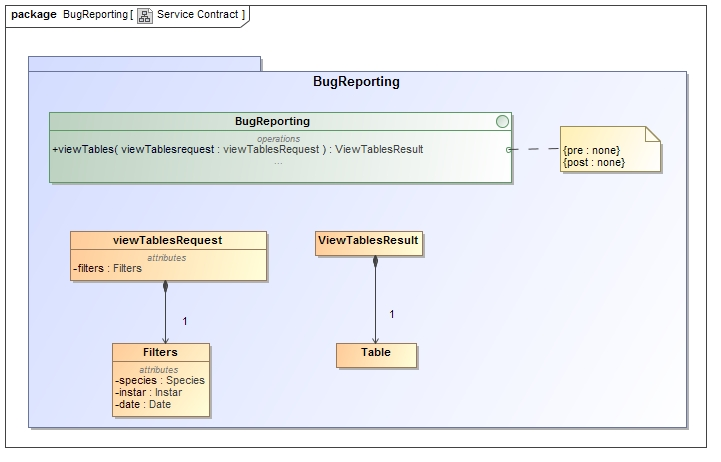
\includegraphics[width=\linewidth]{viewTables}	

	
		
		
\section{Architectural Requirements}
	\subsection{Quality Requirements}
		\subsubsection{Maintainability}
			As a standard requirement for all projects, SAMBUG needs to be maintainable. This is especially due to the fact that the project has very high expansion potential. SUBTROP has shown interest in further maintaining the project after completion.
			Since development on the project is split among 5 members, we have to ensure that the code is as readable as possible and this includes using good documentation of code in the form of comments and Javadoc descriptions.
		\subsubsection{Scalability}
			Since the user base for the system will be comparatively small, scalability is not a great issue. The load on the system will not under any foreseeable circumstances be extremely high. 
		\subsubsection{Performance Requirements}
			Performance is a very important requirement for the system. The goal of the system is to provide an efficient service rendered. Users of the system will be subject to high pressure environments where time is an issue. Using phone memory effectively is also a must as the phones used by the users might not be latest models, and therefore may struggle with some of the more graphical parts of the app.
		\subsubsection{Reliability and Availability}
			Since users will be relying heavily on this system to make important business decisions the system must be available to be used at all times. As such, a reliable system is of paramount importance. The storing of data and persistence of said data to the server must be completely reliable since this is the essential part of the project goal.
		\subsubsection{Security}
			As specified by the client, for the sake of reducing usage complexity of the system, the security may be relaxed in this case due to the fact that the users are generally not comfortable with using technological products. However, security measures should be put in place to help the user navigate through the app in order to complete the data entry process.
		\subsubsection{Auditability}
			There is no specific auditability requirement for the system since there will be no business value in tracking user activity, but for some traceability the user details of someone who edits the database is stored.
		\subsubsection{Testability}
			Every service offered by the system should be testable via:\\
			1. Unit tests\\
			2. Integration tests
		\subsubsection{Usability}
			Usability is the main quality requirement for the system. In order for the system to have any actual business value it should be easy to use and effective. As far as possible, the user should be able to use the app without needing textual instructions.
		\subsubsection{Deployability}
			The system must be deployable to any cloud hosted, Windows based, virtual machine or locally hosted server.
	\subsection{Architecture responsibilities}
	The architectural responsibilities of the system include providing infrastructure for the following:
		\begin{itemize}
			\item A web access channel
			\item A mobile access channel
			\item Hosting for business logic and services offered by the system
			\item Relational database persistence
			\item Sending emails for recovering of accounts
		\end{itemize}
\section{Architectural Design}
	\subsection{Overview}
		A layered architecture will be used to provide for better decoupling of the various		access channels and architectural responsibilities. Within these layers the Model-View-Controller pattern will be applied to further separate concerns among what can be viewed as three distinct parts of a Web application. The following provides an overview of the architecture:
			\begin{itemize}
				\item Access Layer
					\begin{itemize}
						\item View\\
						In many ways the Android application serves as an access channel to the Web server. However, it is not categorised as a "View" in the MVC sense. Our MVC pattern is only used across the Access and Services layers. Therefore, this only encompasses HTML views that are rendered using the Razor rendering engine.
						\item View Model\\
						Model definitions are used both in the View and in the Controller, since these define the primary format of data transfer between those two components. It is important to remember that since MVC is used solely for the frontend, these models are only view models, and not data or domain models.
					\end{itemize}
				\item Services Layer
				    \begin{itemize}
						\item View Model
						\item Web and RESTful Controllers\\
						The MVC Web Controllers communicate with Browser-based clients whilst the RESTful controllers use JSON to communicate with other clients.
						\item Business Logic\\
						Business Logic is extracted from both sets of controllers to allow for common services and for thinner controllers.
					\end{itemize}
				\item Data Access Layer
				    \begin{itemize}
						\item Domain Model						
						\item Data Abstraction (Repository)\\
						This interface defines a contract between the application and the database, allowing us to swap our current database implementation for any other implementation that realises the contract. Query methods map entities to domain models which are returned to the Services layer for further processing. This further decouples our domain from our data.
						\item MSSQL Implementation\\
						This is our current Database implementation. Entity Framework is used as an ORM. Entities are defined here and are used to query the database with LINQ.						
					\end{itemize}
			\end{itemize}
	\subsection{Infrastructure Layout}
		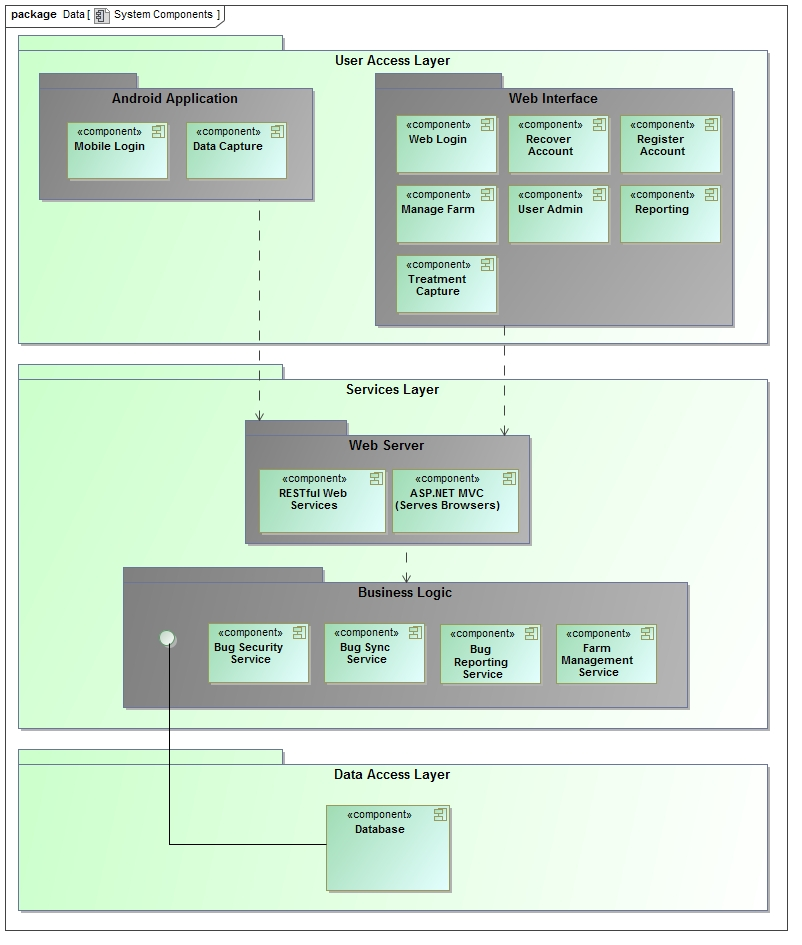
\includegraphics[width=\linewidth]{SystemComponents}	
	\subsection{Database Design}
	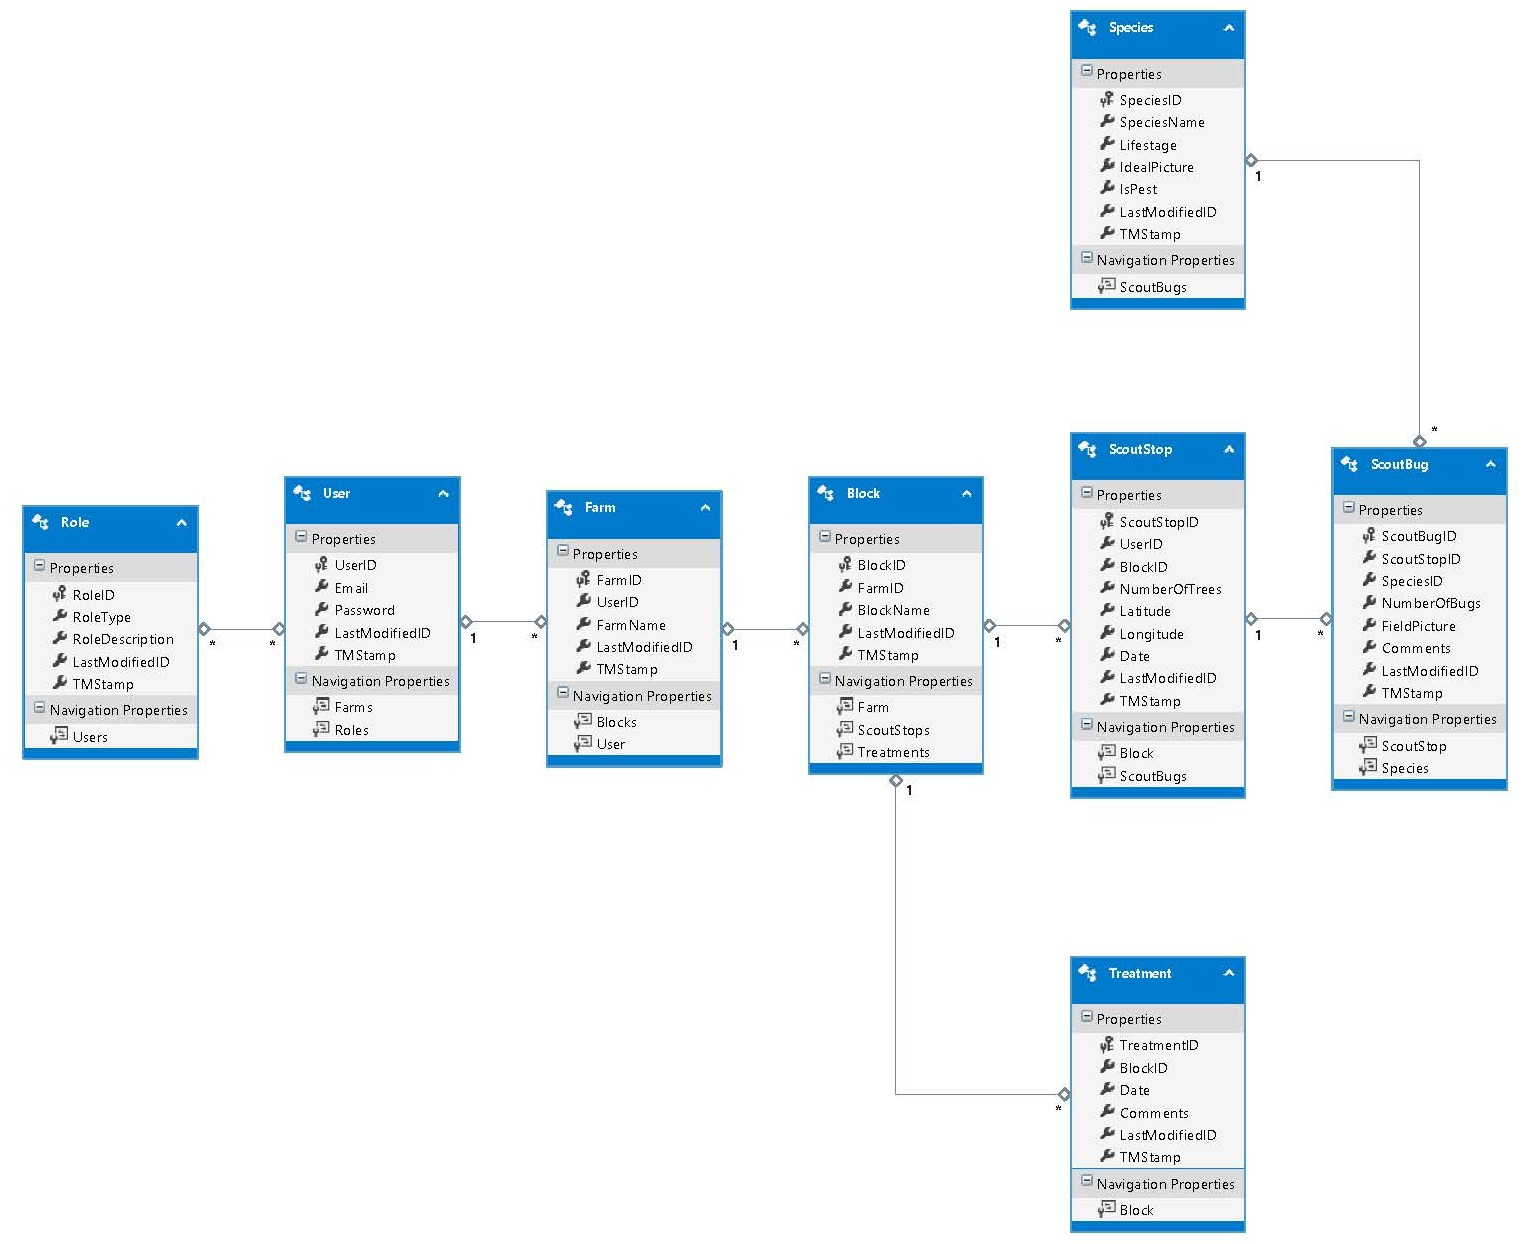
\includegraphics[width=\linewidth]{ERD}	
	\subsection{Process Flow}
		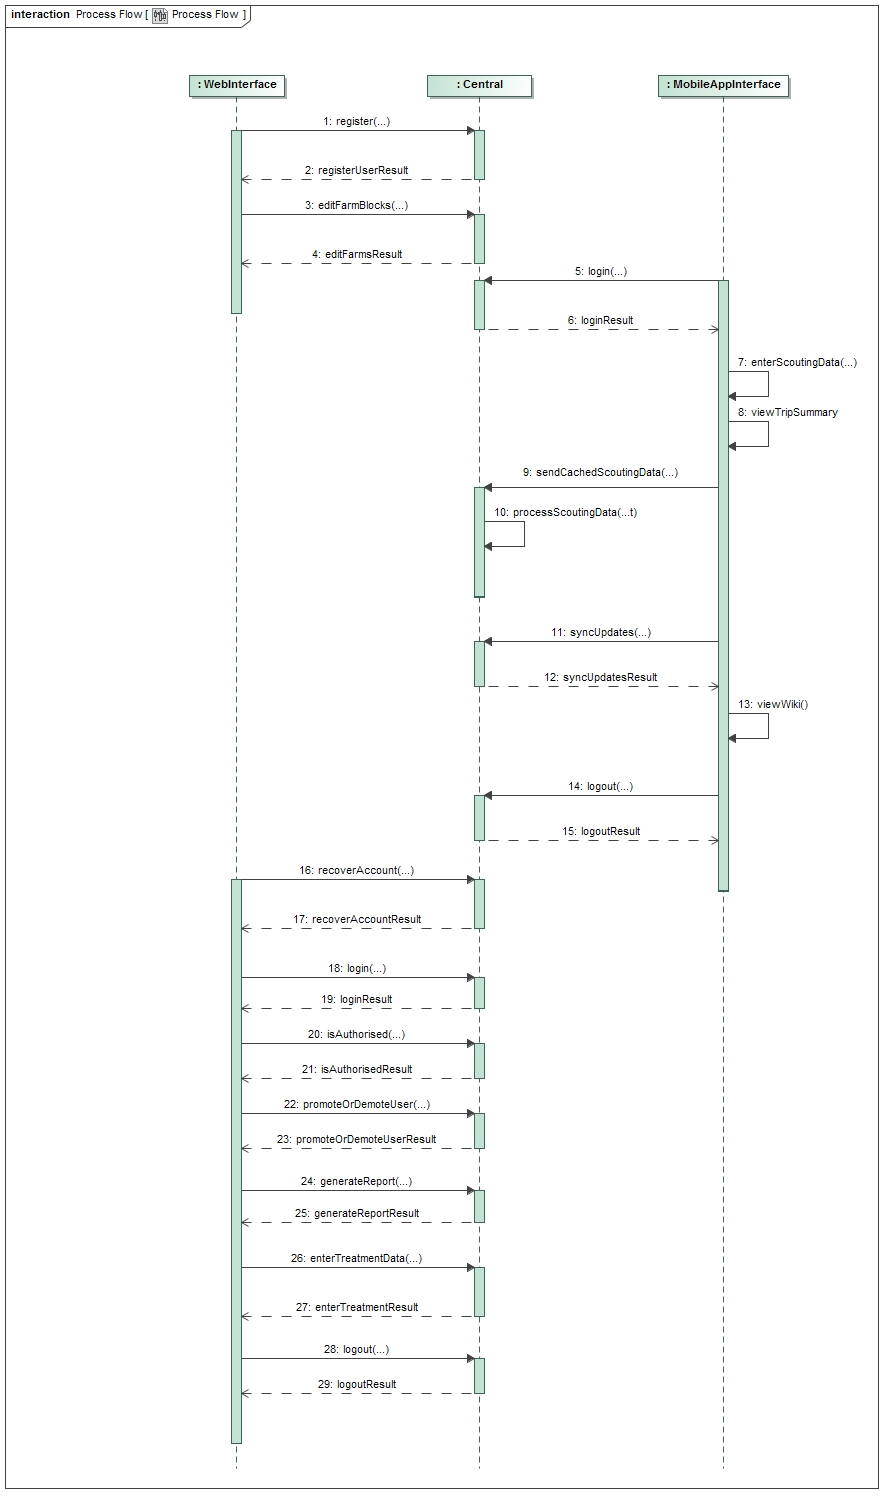
\includegraphics[width=\linewidth]{ProcessFlow}	
	\subsection{Technologies}
		\subsubsection{Mobile Application}
			\paragraph{Android Studio}
				 We chose to use this development suite because of the following:
				\begin{itemize}
				\item It is the industry standard for Android app development.
				\item The IDE provides lots of code analysis with the tool named Lint. It also has a very good dynamic layout preview to design the interfaces for specific screen variations.
				\item Furthermore, we decided to develop the app natively instead of using a cross-platform alternative like Titanium because the client specified that only an Android app would be required and therefore it seems pointless to deal with hassles that may arise in cross-platform development. 
				\item A large focus for our group, specifically in the mobile app, is a high quality user interface. This particular aspect is something we stand to lose if we develop for cross-platform since we would only be able to use common controls between Android and iOS, for example.\end{itemize} 
				For more information regarding Native vs. Cross-platform development, click \href{https://yalantis.com/blog/native-vs-cross-platform-app-development-shouldnt-work-cross-platform/}{here}.
			\paragraph{Mockito}
		There are many Mocking Frameworks available for Android App development. 
		Mockito stands out from the others in the following respects:
			\begin{itemize}
				\item Mockito is simple to use, implement and is a lot more readable, especially when compared to the likes of RhinoMock, JMockit and EasyMock. These other frameworks are are old, unpleasant and difficult to find documentation for.
				\item Mockito not only allows interfaces to be mocked, but also allows abstract and concrete classes to be mocked. Furthermore, this can be done without any extensions (e.g. EasyMock requires class extentions.)
				\item Since it is a single Jar file, it is easy to setup. 
				\item Mockito supports spies (to create partial mocks), in order to gather indirect output from a test, meaning functions can be tested and verified without giving the test input. 
				\end{itemize}
				For more information regarding Mockito vs. EasyMock, click \href{https://code.google.com/p/mockito/wiki/MockitoVSEasyMock}{here}. \newline
				For more information regarding the pros and cons of Mockito, click \href{http://hamletdarcy.blogspot.com/2010/09/mockito-pros-cons-and-best-practices.html}{here}. \newline
				For more information regarding Mockito vs. PowerMock/JMockit, click \href{http://www.coderanch.com/t/524265/Testing/TestNG-JUnit-mockito-Powermock-jmockit}{here}. \newline

			\paragraph{SQLite}
				SQLite is a relational database management system which is contained in a C programming library. It was selected because of the following: 
					\begin{itemize}	
						\item It is available for free. 
						\item It is Portable, because the whole database is located on a single file making easy to transfer.
						\item It is easy to query data, because data is stored in a simple structured way.
						\item SQLite has higher performance than many other relational db management systems and uses a low amount memory.
						\item It is easier to manage since there is no file parsing and generated code that needs to be debugged. 
						\item The content can easily be viewed using various third-party tools.
					\end{itemize}
For more information regarding a comparison of SQLite and other relational db management systems, click \href{https://www.digitalocean.com/community/tutorials/sqlite-vs-mysql-vs-postgresql-a-comparison-of-relational-database-management-systems}{here}. \newline
For more information regarding why SQLite is used in Android App Development, click \href{http://www.quora.com/Why-should-we-use-SQLite-in-Android-development}{here}. \newline
		\subsubsection{Web Backend}
			\paragraph{.NET WebAPI}
				The Microsoft .NET framework was chosen as a backend framework for hosting RESTful services. The following factors contributed to this decision:
				\begin{itemize}
					\item The .NET framework is a tried and tested industry standard technology which adds value to the Reliability component of the 
							quality requirements.
					\item The .NET framework and packages used within the project became open source as announced by Microsoft at the Build 214 conference thus freeing the client from licensing fees. See the \href{http://www.dotnetfoundation.org/projects}{.NET Foundation}  for further details on open source Microsoft Packages.
					\item The main alternative to the .NET framework was the Java EE reference framework. Since Performance and Scalability is a very important quality requirement .NET was deemed superior due to case studies consulted:
							\begin{itemize}
								\item  \href{http://www.slideshare.net/tejasvirastogi/java-vs-net-24443514}{Testing .NET vs Java EE with basic web pages}
								\item  \href{http://www.seguetech.com/blog/2013/06/03/dotnet-vs-java-how-to-pick}{How to pick between Java and .NET}
								\item  \href{http://stackoverflow.com/questions/18088/are-there-any-studies-comparing-java-ee-vs-net}{.NET vs Java Discussion}
							\end{itemize}
							It is worth noting that Java EE and .NET are very closely matched in many aspects. The difference between the two frameworks are nearly negligible in terms of performance.
					\item The .NET framework provides seamless integration with the other technologies utilised
					\item The .NET framework provides for quick and easy set-up for REST services and web front ends using MVC5		
				\end{itemize}
			\paragraph{AutoMapper}
				AutoMapper is used to do automated maping from DTO's (Domain Transfer Objects) to Domain (or Data) objects, and vice versa. This is simply used to promote code reusability and readability.
			\paragraph{.NET MVC 5}
				For the same reasons mentioned for the choice of .NET WebAPI. MVC 5 was chosen as a pattern at a lower level of granularity due to the built in support for it in the .NET framework and it can be viewed in most cases as a industry standard for web applications.
			\paragraph{MSSQL Express}
					Express is the free version of the Microsoft RDBMS which caters for all the data needs of the system. This technology can easily be swopped out for other free database technologies such as MySQL
					due to the technology neutral architecural design.
			\paragraph{AutoFac}
					AutoFac is used as a mocking framework for unit testing as well as for dependency injection in order to fascilitate more effective unit testing and pluggability. Using this dependency injection framework code maintainability is also improved.
		\subsubsection{Web Frontend}
			\paragraph{DataTables}
				DataTables is a plug-in for the popular jQuery Javascript library. It enables powerful DOM manipulation and data-binding specifically for data-driven web pages. Since the SAMBUG Website mainly features a dashboard that enables growers to peer into their bug collection and treatment history, tables and charts will be at the heart of the Web front-end. This library is specifically for dynamic table creation from multiple data sources.
			\paragraph{Chartist-js}
				Chartist is a JavaScript charting library providing flexible and responsive charts for our Reporting Module. Chartist prefers convention over configuration and although it's compact and focused at its core, its functionality may be extended via plug-ins. This libary draws its chart elements in the Scalable Vector Graphics format, allowing crisp images, independent of device specifications. 
			\paragraph{AngularJS}
				Angular is the next generation JavaScript client framework for mobile, desktop and web. It provides two-way databinding (as does Aurelia.io) and extensible HTML as well as other great features such as client side dependency injection
				. Angular is the way forward for client side scripting frameworks. The other major competitor in this area is AureliaIO. See \href{http://ilikekillnerds.com/2015/01/aurelia-vs-angularjs-round-one-fight/}{Aurelia vs AngularJS – Round One: FIGHT!}
		\subsubsection{Builds and Deployment}		
			\paragraph{AppHarbor}
				This is a hosted .NET Platform as a Service. AppHarbor attaches to our version control system (Git) and monitors commits to the master branch. It automatically builds the latest source, runs unit and integration tests and finally deploys when the tests have all succeeded. AppHarbor also hosts our MSSQL development database.
			\paragraph{Gradle}
				This build system is the standard for Android Studios and therefore it allows us to easily get apps built and running. Testing and debugging apps is made really simple using Gradle. It also allows us to perform incremental building. 
			\paragraph{MSBuild}
				MSBuild is the standard build script language for the .NET development environment. Since it functions seamlessly there is no need to change this technology.
		\subsubsection{Testing}
			\paragraph{JUnit}
				Junit was selected as the Unit Testing framework because:
					\begin{itemize}	
						\item It is simpler to use and has better online documentation than competitors such as TestNG.
						\item Junit is the most popular testing framework in Industry. 
						\item It is easy to integrate Junit as part of your build process. 
						\item Since it is the most popular testing framework,  new features are constantly  being added.
					\end{itemize}
For more information on why JUnit was chosen compared to other Testing Frameworks, click \href{http://blog.javafortesters.com/2014/09/faq-should-i-use-junit-or-testng-which.html}{here} and
\href{https://seleniumonlinetrainingexpert.wordpress.com/2012/11/21/what-are-advantages-of-testing-with-junit/}{here.} \newline

			\paragraph{MSTest}
				MSBuild is the standard testing pacakge for the .NET development environment. Since it functions seamlessly there is no need to change this technology.
		
	\subsubsection{Artifical Intelligence and Computer Vision}
		\paragraph{OpenCV}
			OpenCV is a open source library which focuses on computer vision applications and artifical intelligence. It is believed to be the most popular and reliable open source library in the field. The OpenCV library was used for preprocessing of images for the neural network which is also supplied via OpenCV. EmguCV was used as .NET bindings for the OpenCV library. 

	\subsubsection{Additional Technologies}
		\paragraph{Fiddler 4}
			Fiddler is a .NET orientated debugging program similar to WireShark which is used to monitor HTTP requests and set up custom requests to any specified server in almost any specific form (GET, POST, PUT etc.)
		\paragraph{Git and GitHub}
			Git is the version control system of choice which is utilised for the system. The public repository from whch the code base is hosted is named GitHub and may be accessed at \url{https://github.com/WMostert1/Vector-Software-Developers}.
		\paragraph{Material Design}
			Material Design is a design language that was developed by Google used to make the experience of viewing a mobile or web application more real and alive. We have decided with this technology as we believe it can make our system only better, especially when Material Design and implementations thereof has had time to grow. We believe it can make our system visually more appealing and also make our system more accessible.
			
			Angular Material will be used on the web interface. Angular material is an implementation of Material Design.  
		\paragraph{Misc. Javascript Frameworks and Libraries}
			Various, mostly JavaScript, libraries are utilised for the reporting services and user interface.
%\section{Open Issues}


%\pagebreak
%\section{Notifications and Messages Domain}
%  \input{Notifications}

\end{document}